\section{Homographies}

Sometimes there are photographies of the same object but taken from different perspectives (Fig. \ref{fig:homog}). 

\begin{figure}[H]
    \centering
    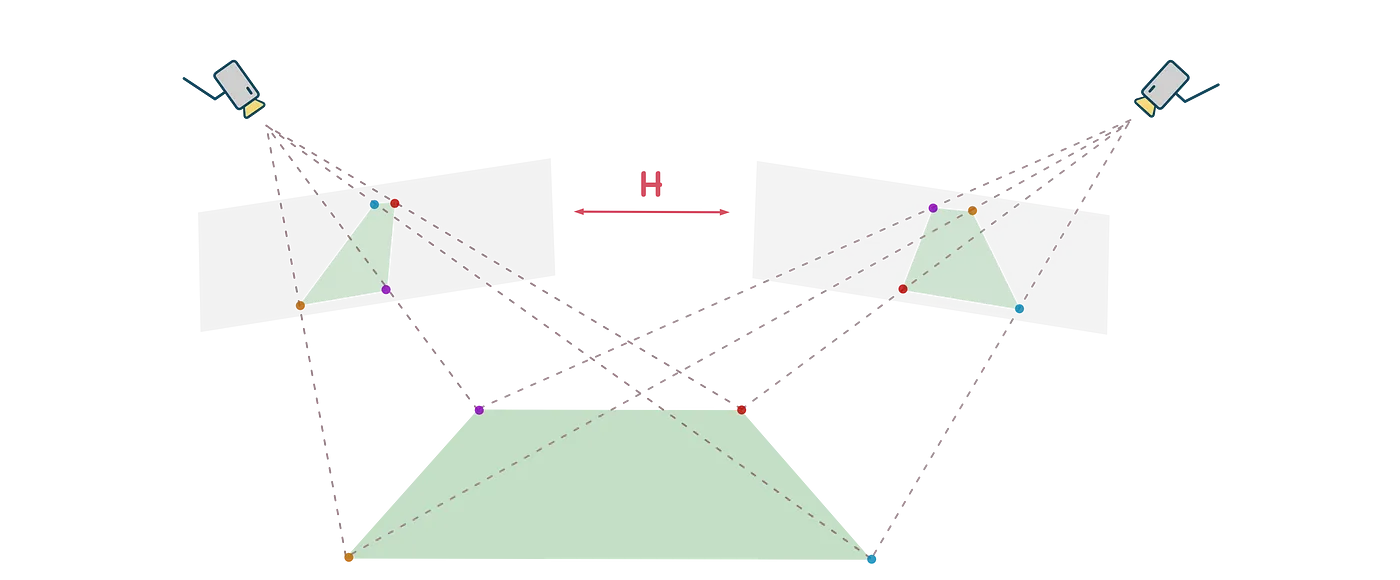
\includegraphics[width=0.8\textwidth]{img/homog}
    \caption{Different perspectives of the same object \cite{noauthor_opencv_nodate}}
    \label{fig:homog}
\end{figure}

The concept of homography raises with the aim of represent how each point can be converted into other (because in reality they are the same point). To represent this spacial translation, a function can be used, and this function can be represented as a matrix.

\begin{gather*}
    \lambda
    \begin{bmatrix}
        x' \\ y' \\ 1
    \end{bmatrix} = 
    \begin{bmatrix}
        H_{1,1} & H_{1,2} & H_{1,3} \\
        H_{2,1} & H_{2,2} & H_{2,3} \\
        H_{3,1} & H_{3,2} & H_{3,3}
    \end{bmatrix}
    \begin{bmatrix}
        x \\ y \\ 1
    \end{bmatrix}
\end{gather*}


